% !TEX root = master_thesis.tex

%==============================================================================
\chapter{Introduction}
\newcommand{\btheta}{\boldsymbol{\theta}}
\label{chap:intro}
%This chapter will give a brief introduction into the theoretical concepts that motivate this work. First the Standard Model of Particle Physics is sketched along with characteristics of the strong interaction. Next, the photoproduction of mesons and the importance of polarization observables is explained. Lastly the particular motivation and structure of this work will be presented.
%==============================================================================
%\section{The Standard Model of Particle Physics}
The \emph{Standard Model of Particle Physics} (SM) is the most successful model aiming to describe the particles and forces of the universe. It distinguishes between \emph{fermions} and \emph{bosons}. While all matter consists of fermions, bosons are particles that mediate the fundamental interactions.

Matter consists of (anti-)quarks and (anti-)leptons with three generations of each. Table \ref{tab:sm0} shows all elementary fermions including some of their most important properties. Only the first and lightest generation consists of stable particles, i.e. the up and down quark as well as the electron and its neutrino. All other particles are heavier and not stable, they will thus decay fast via the strong, electromagnetic or weak interaction.

There are in fact four interactions described by the SM: strong, electromagnetic, weak and gravitational interaction \footnote{they are ordered here according to their relative strength}, where gravitation is mentioned here for the sake of completeness; on the mass scale of elementary particles gravitation is negligible. Strong and weak interaction are restricted to a finite range of the order of the nucleon radius, whereas electromagnetic interaction and gravitation have infinite range. Each interaction has its own coupling (charge). The strong interaction is mediated by gluons and couples to the color charge.% A summary of the SM interactions can be found in table \ref{tab:sm1}.
\begin{table}[htbp]
	\centering
	\begin{tabular}{cccccc}
		\toprule
		&\multicolumn{3}{c}{\textbf{Generation}}&\textbf{el. charge}&\textbf{color charge}\\
		&\textbf{1} & \textbf{2} & \textbf{3} & & \\
		\hline
		\textbf{Quarks} & $u$&$c$&$t$& 2/3 & r,g,b\\
		&$d$&$s$&$b$& 1/3 & r,g,b\\
		\textbf{Leptons}& $e$&$\mu$&$\tau$&-1& -\\
		& $\nu_e$&$\nu_\mu$&$\nu_\tau$&0&-\\
		\bottomrule

	\end{tabular}
\caption{Summary of the particles of the SM}
\label{tab:sm0}
\end{table}
%\begin{table}[htbp]
%	\centering
%	\begin{tabular}{ccc}
%		\toprule
%		interaction & couples to & Gauge boson\\
%		\hline
%		strong & color & $g$\\
%		elm.& el. charge & $\gamma$\\
%		weak&weak charge & $W^\pm,Z^0$\\
%		\bottomrule
%	\end{tabular}
%
%	\caption{Summary of the interactions of the SM}
%	\label{tab:sm1}
%\end{table}



Gluons and quarks carry color charge and thus interact strongly. However, an isolated quark or gluon has not been observed. Only color neutral bound systems of quarks are seen, which are called hadrons. Hadrons with integer spin are called mesons and those with half-integer spin are called baryons. Color neutrality demands mesons consist of at least one quark and one anti-quark and baryons consist of at least three quarks.


 As already mentioned, isolated quarks are not seen. This can be understood in terms of the strong coupling constant $\alpha_s$. The coupling constant is a measure of the strength of the strong interaction. Because it is highly dependent on the momentum transfer in the observed strong reaction it is also called running coupling constant, which is depicted in figure \ref{fig:coupl}.
 \begin{figure}
 	\centering
 	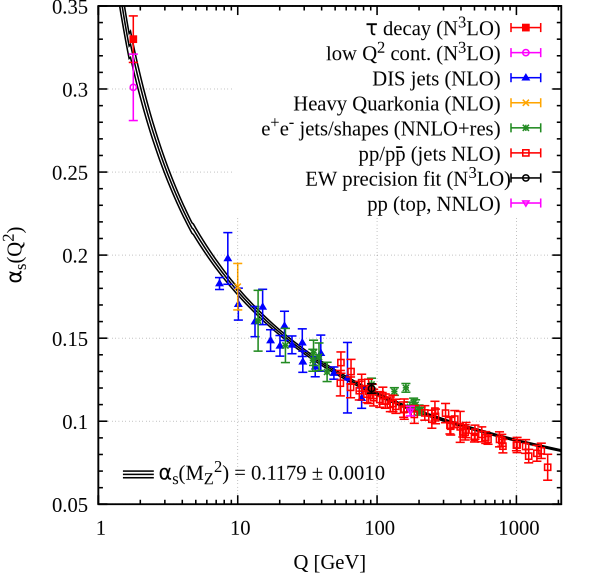
\includegraphics[width=.5\linewidth]{qcd}
 	\caption{Running coupling of QCD. The colored data points represent different methods to obtain a value for $\alpha_s$. For a detailed review see \cite{pdg}.}
 	\label{fig:coupl}
 \end{figure}

 For low ($<\SI{1}{\GeV}$) momentum transfers or large distances the coupling constant approaches infinity whereas it decreases for high ($\gg\SI{1}{\GeV}$) momentum transfers or short distances. These momentum ranges are referred to as \emph{confinement} and \emph{asymptotic freedom}, respectively; quarks are confined to remain in a bound state since if one tried to pull them apart the color field becomes so strong it will create a new quark anti-quark pair resulting in two new bound states. On the other hand, bound quarks behave quasi-free and can be described using perturbative quantum chromodynamics (pQCD) if probed at sufficiently large momentum transfers.

 It is more difficult however to describe QCD at momentum scales of $\approx \SI{1}{\GeV}$ since the coupling is too strong to justify a perturbative approach. Thus explicit modeling of QCD bound states is inevitable. One possibility is to describe baryons consisting of constituent quarks which are bound in a potential. Constituent quark models assume baryons are made up of three constituent quarks with effective masses differing from the bare quark mass. The effective mass is made up mostly from a sea of quark anti-quark pairs and gluons which surround the bare (valence) quarks. The explicit form of the binding potential is determined for each model.

 The Bonn model \cite{bonnmodel}, for example, is formulated as a relativistically covariant constituent quark model.
 A potential increasing linearly with the distance is employed to adequately describe confinement. The binding potential between the constituent quarks is described by an instanton-induced interaction. Baryon resonances are then states with an orbital or angular excitation of one of the quarks. Figure \ref{fig:bm} shows computed  nucleon resonances with Isospin $I=1/2$ of the Bonn model \cite{bonnmodel} on the left side of each column. These are compared to measured resonances and their PDG rating \cite{pdg} in the middle. Uncertainties are indicated by the colored areas. The resonances are identified by their total angular momentum and their parity $J\pi$. In addition also the total internal angular momentum along with isospin and again the total angular momentum $L_{2T2J}$ is given.
  \begin{figure}[htbp]
 	\centering
 	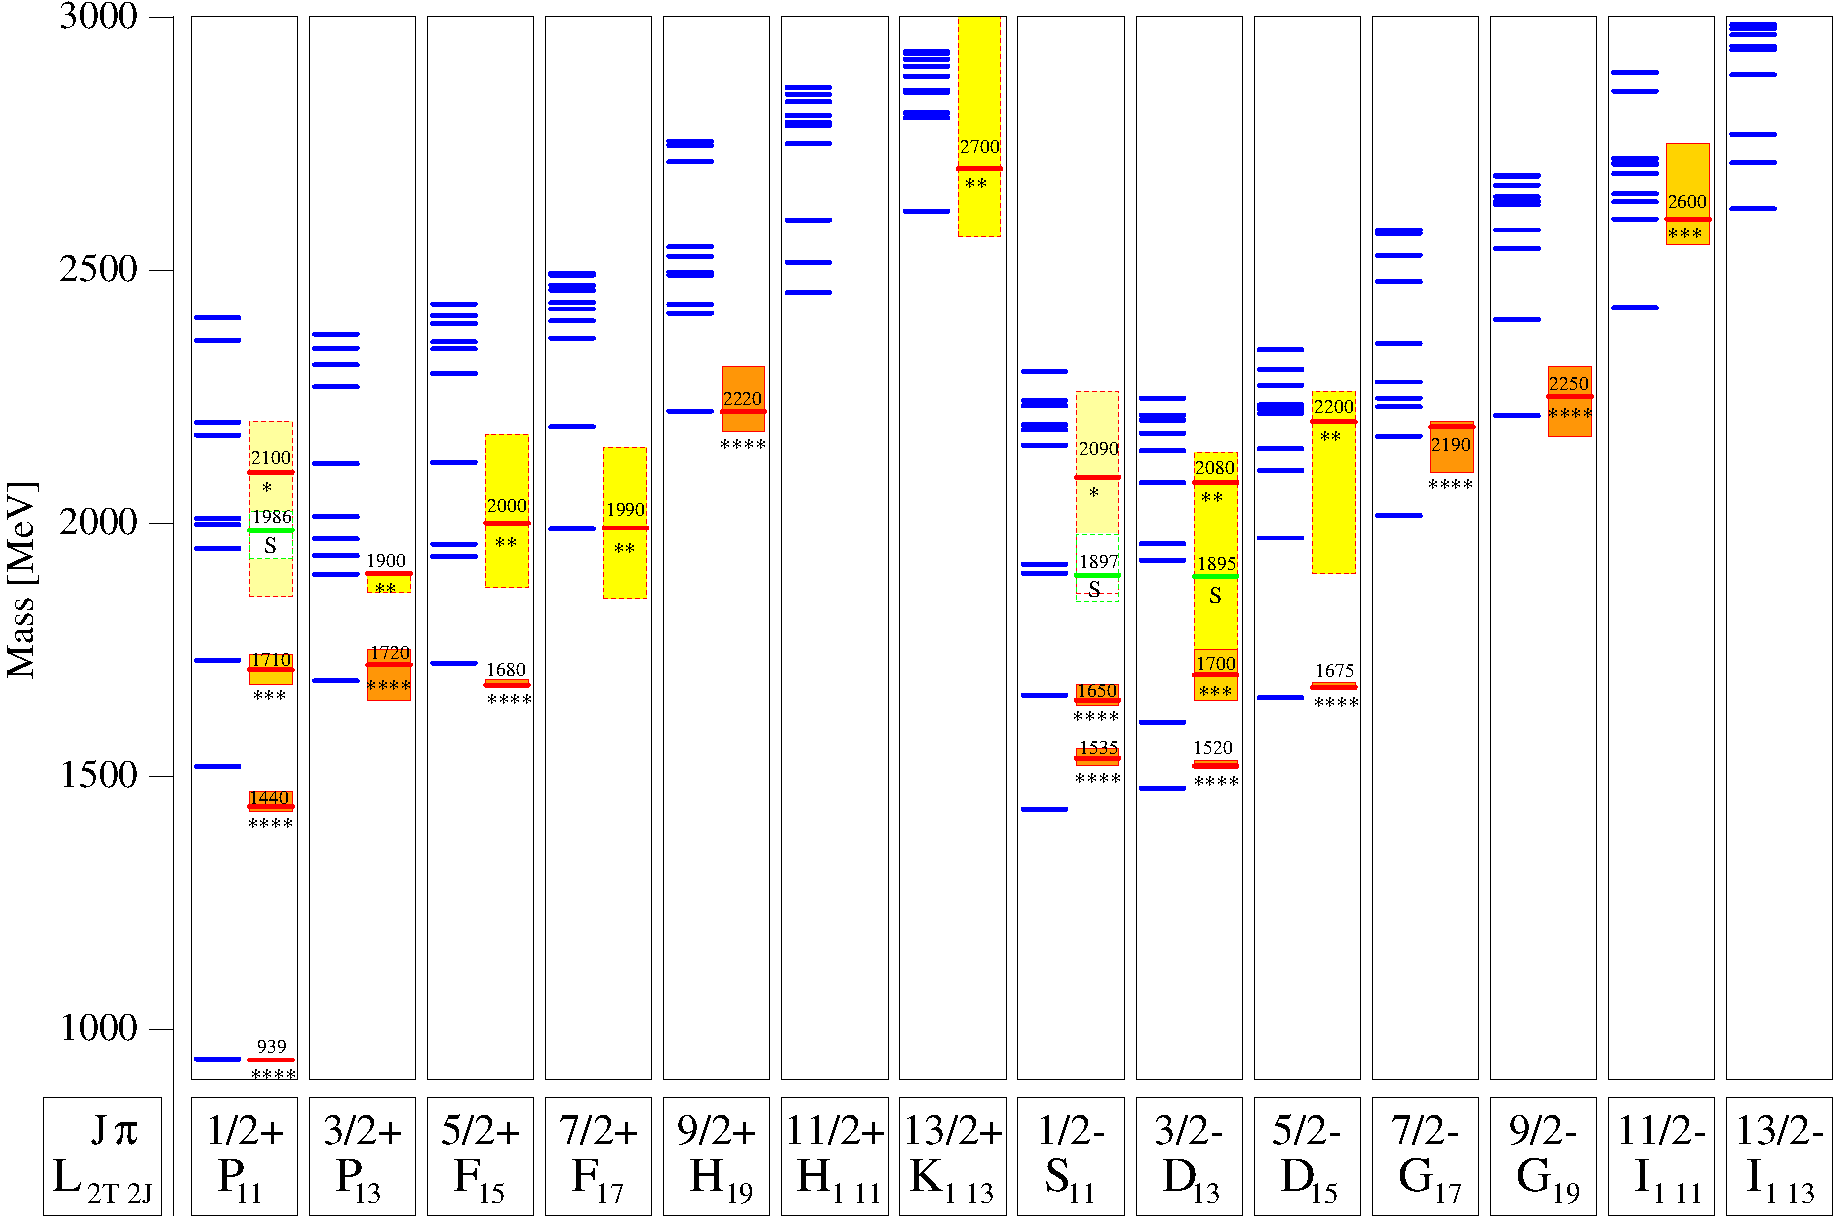
\includegraphics[width=\linewidth]{figs/NucM2.pdf}
 	\caption{Calculated nucleon (isospin $I=1/2$) resonances compared to measurements. Left in each column are the calculations \cite{bonnmodel}, the middle shows the measurements and PDG rating \cite{pdg}}
 	\label{fig:bm}
 \end{figure}
While generally good agreement exists for low lying resonances, especially for high masses there are much more resonances predicted than actually found. This is also known as the problem of the \enquote{missing resonances} indicating the poor understanding of QCD in the non-perturbative region. This can be due to several reasons: most of the knowledge about nucleon resonances and their properties was obtained investigating the $\pi N$ channel, biasing the data for resonances coupling weakly to this channel. Furthermore, the number of excited states with definite quantum numbers is related directly to the effective number of degrees-of-freedom accessible to the underlying theory. As a consequence, the number of degrees-of-freedom should be obtainable by comparing the measured states to the predicted states. Since nucleon resonances decay dominantly hadronic, their resonances are broad and overlapping. Thus on one hand the determination of excitation spectra proves to be a challenge on its own, demanding sophisticated methods, such as partial wave analysis (PWA). On the other hand it is not yet clear how many effective degrees-of-freedom exist for the nucleon in a constituent quark model. They could for example be decreased if the nucleon were made up of a quark and a di-quark structure. To access nucleon resonances and transitions between them for as many final states as possible the photoproduction of mesons off the proton has gained attention. Experiments dedicated to study photoproduction reactions off nucleons are located e.g. at JLAB, MAMI or ELSA. In this thesis photoproduction data taken at the CBELSA/TAPS experiment, which is located at the accelerator ELSA in Bonn, is analyzed regarding the reactions $\gamma p \to p \eta$ and $\gamma p \to p \eta'$. The theoretical foundation underlying the photoproduction of pseudoscalar mesons and the measurement of polarization observables will be discussed in the next sessions.
\section{Photoproduction of Pseudoscalar Mesons}
From the scattering theory point of view, photoproduction of mesons is well understood \cite{Krusche}. Figure \ref{fig:mes_bildchen} shows schematically the process thereof off the proton:

\begin{figure}[htbp]
	\centering
	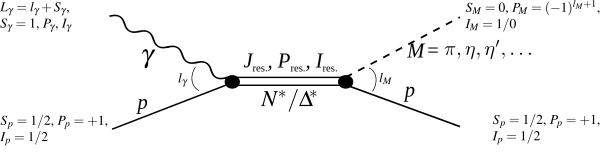
\includegraphics[width=\linewidth]{meson_bildchen}
	\caption{\textsc{Feynman} diagram for the s-channel photoproduction of pseudoscalar mesons, adapted from \cite{farahphd}}
	\label{fig:mes_bildchen}
\end{figure}

The analysis requires partial wave decomposition in both initial and final states \cite{Drechsel} since the intermediate resonance $N^*/\Delta^*$ has definite angular momentum, parity  and isospin $J_\text{res.}, P_\text{res.}, I_\text{res.}$. The resonance is excited by a photon with (iso-) spin $I_\gamma,S_\gamma =1$ and parity $P_\gamma$ coupling electromagnetically to the target proton with (iso-) spin $I_p=1/2,S_p=1/2$ and parity $P_p$. The relative momentum is $l_\gamma$, such that the total momentum of the photon is $L_\gamma=l_\gamma+S_\gamma$. The parity of the photon depends on the multipolarity of the photon and is given by $P_\gamma=(-1)^{L_\gamma}$ for electric ($E$) or $P_\gamma=(-1)^{L_\gamma+1}$ for magnetic ($M$) photon multipoles \cite{Drechsel}. Subsequently the intermediate state will have the quantum numbers $J_\text{res.}, P_\text{res.}, I_\text{res.}$ and decay into a proton with spin $S_p=1/2$, parity $P_p=+1$ and isospin $I_p=1/2$ under emission of a meson. Here, only pseudoscalar mesons that have vanishing spin $S_M=0$, isospin $I_M$, relative orbital angular momentum $l_M$ und Parity $P_M=(-1)^{l_M+1}$ are considered. Note that for $\eta$ and $\eta'$ mesons $I_M=0$; this exclusively limits the intermediate resonances to $N^*$ states since the strong interaction conserves isospin \cite{pdg}. The following selection rules can be derived using parity and momentum conservation \cite{Krusche,farahphd}
\begin{align}
	%\left|L_\gamma-S_p\right|&=\left|L_\gamma-1/2\right|\leq J_\text{res.}\leq\left|L_\gamma+1/2\right|=\left|L_\gamma+S_p\right|,\\
	J_\text{res.}&=L_\gamma\oplus S_p = L_\gamma\oplus 1/2,\\
	P_\text{res.}&=P_p\cdot P_\gamma=P_\gamma,\\
	%\left|l_M-S_p\right|&=\left|l_M-1/2\right|\leq J_\text{res.}\leq\left|l_M+1/2\right|=\left|l_M+S_p\right|,\\
	J_\text{res.}&=l_M\oplus S_p = l_M\oplus 1/2\\
	P_\text{res.}&=P_p\cdot P_M=(-1)^{l_M+1},
\end{align}
where the usual rules for the coupling $\oplus$ of angular momenta \cite{theo3} apply. Thus, knowledge of the photoproduction multipoles allows the identification of contributing resonances for particular mesonic final states. Table \ref{tab:qn} shows a summary of allowed quantum numbers according to the shown selection rules for the lowest order of photon multipoles ($L_\gamma=1$). The photoproduction multipoles $E_{l\pm},M_{l\pm}$ indicate the relative momentum of the meson ($l=l_M$) and whether the total angular momentum is obtained by adding \enquote{+} or substracting \enquote{--} the final state momenta. Resonances are identified in spectroscopic notation by the meson momentum $l_M$ as well as by their (iso-)spin $I,J$ and Mass $M$. Note that only $2I=1$ resonances are listed since the mesons $\eta$ and $\eta'$ have vanishing isospin, so that only $I=1/2$ resonances ($N^*$ resonances) may be accessed.
\begin{table}[htbp]
	\centering
	\begin{tabular}{cccccc}
		\toprule
		\textbf{Photon}   & \textbf{initial state} & \textbf{intermed.} & \textbf{final state} & \textbf{photoproduction}&\textbf{resonance}\\
		 \textbf{multipole}& $\boldsymbol{\left(L_\gamma^{P_\gamma}, S_p^{P_p}\right)}$ & \textbf{state} $ \boldsymbol{J_\text{res}^{P_\text{res}}}$& $\boldsymbol{\left(S_p^{P_p},l_M^{P_M}\right)}$ & \textbf{multipole} $\boldsymbol{E_{l\pm}, M_{l\pm}}$ & $\boldsymbol{\left(l_M\right)_{2I2J} (M)}$\\
		 \hline
		 $E1$ & $\left(1^-,\frac{1}{2}^+\right)$ & $\frac{1}{2}^-$ &$\left(\frac{1}{2}^+,0^-\right)$&$E_{0+}$& $S_{13}(M)$\\
		 $E1$ & $\left(1^-,\frac{1}{2}^+\right)$ & $\frac{3}{2}^-$ &$\left(\frac{1}{2}^+,2^-\right)$&$E_{2-}$& $D_{13}(M)$\\
		 $M1$ & $\left(1^+,\frac{1}{2}^+\right)$ & $\frac{1}{2}^+$ &$\left(\frac{1}{2}^+,1^+\right)$&$M_{1-}$& $P_{11}(M)$\\
		 $M1$ & $\left(1^+,\frac{1}{2}^+\right)$ & $\frac{3}{2}^+$ &$\left(\frac{1}{2}^+,1^+\right)$&$M_{1+}$& $P_{13}(M)$\\
		 \bottomrule
	\end{tabular}
\caption{Allowed quantum numbers for the intermediate resonance state $N^*$ in $\eta/\eta'$-photoproduction. Adapted from \cite{farahphd}}
\label{tab:qn}
\end{table}
The determination of contributing multipoles which can then be used to identify nucleon resonances is challenging and requires sophisticated (model dependent) partial wave analyses (PWA). The measurement of polarization observables helps to eliminate ambiguities in PWA calculations as will be explained in the following section.
\section{Measurement of Polarization Observables}
Using an ansatz purely motivated by scattering theory, the differential cross section of meson photoproduction can be written as 
\begin{equation}
	\frac{\text{d}\sigma}{\text{d}\Omega}=\frac{q}{k}\left|\braket{f|\mathcal{F}|i}\right|^2,
	\label{eq:cs}
\end{equation}
where the matrix element is taken between initial and final \textsc{Pauli} spinors \cite{cgln} and $q$ and $k$ denote the momentum of the incident photon and final state meson, respectively. The photoproduction amplitude $\mathcal{F}$ contains all relevant information regarding the scattering process connecting the initial and final state in analogy to the $S$-matrix that is introduced in the general discussion of quantum-mechanical scattering \cite{ps}. Following the notation of reference \cite{cgln} it can be written as a sum of the complex \textsc{Chew-Goldberger-Low-Nambu} (CGLN) amplitudes $F_i$
\begin{equation}
	\mathcal{F}=i(\vec{\sigma} \cdot \vec{\epsilon}) F_{1}+(\vec{\sigma} \cdot \hat{q})(\vec{\sigma} \cdot(\hat{k} \times \vec{\epsilon})) F_{2}+i(\vec{\sigma} \cdot \hat{k})(\hat{q} \cdot \vec{\epsilon}) F_{3}+i(\vec{\sigma} \cdot \hat{q})(\hat{q} \cdot \vec{\epsilon}) F_{4},
\end{equation}
where $\hat{k}$ and $\vec{\epsilon}$ are the momentum unit vector and polarization vector of the incident photon, $\hat{q}$ is the momentum unit vector of the final state meson and $\vec{\sigma}$ denote the \textsc{Pauli} matrices. Applying the method of partial waves onto the complex CGLN amplitudes $F_i$ one can absorb the angular dependence into \textsc{Legendre} polynomials $P_l(\cos\theta)$ and derivatives thereof \footnote{Here $\cos\theta$ denotes the polar angle of the meson in the center of mass system} and express the energy dependence solely by the photoproduction multipoles $E_{l\pm},M_{l\pm}$, e.g. for $F_1$ one finds\cite{cgln}
\begin{equation}
	F_{1}=\sum_{l=0}^{\infty}\left[l M_{l+}(W)+E_{l+}(W)\right] P_{l+1}^{\prime}(\cos \theta)+\left[(l+1) M_{l-}(W)+E_{l-}(W)\right] P_{l-1}^{\prime}(\cos \theta),
	\label{eq:f1}
\end{equation}
where $W$ is the center of mass energy. Inserting the partial wave expansion of all CGLN amplitudes into Equation \eqref{eq:cs} directly connects the CGLN amplitudes and the photoproduction multipoles to the cross section which is a measurable quantity. However, the measurement of the differential cross section will give one real number which is not sufficient to unambigously determine four complex amplitudes. To be able to access further observables that are connected to the CGLN amplitudes and the photoproduction multipoles, a polarized target and/or a polarized photon beam can be employed. In total, one may measure 16 non-redundant polarization observables \cite{san} that are grouped into four categories: single polarization observables, where either the beam photon, target proton or recoil proton are polarized, and three groups of double polarization observables where two of the mentioned particles are polarized, i.e. the three groups are beam-target (BT), beam-recoil (BR) and target-recoil (TR) observables. In Table \ref{tab:pol} all single and double polarization observables in pseudoscalar meson photoproduction are listed. Eight carefully chosen observables allow an unambigous determination of all CGLN amplitudes \cite{chiang}, which are then referred to as a \emph{complete experiment} \cite{chiang,san}.
\begin{table}[htbp]
	\centering
	\begin{tabular}{c|cccc}
	\toprule
		\textbf{category}&\multicolumn{4}{c}{\textbf{observables}}\\
		\hline
		non /single & $\frac{\text{d}\sigma}{\text{d}\Omega}$ / & $\Sigma$ &$T$&$P$\\
		beam-target&$G$&$H$&$E$&$F$\\
		beam-recoil&$O_{x'}$&$O_{z'}$&$C_{x'}$&$C_{z'}$\\
		target-recoil&$T_{x'}$&$T_{z'}$&$L_{x'}$&$L_{z'}$\\
		\bottomrule
	\end{tabular}
\caption{All 16 non redundant polarization observables in pseudoscalar meson photoproduction \cite{san}. Table adapted from \cite{farahmsc}.}
\label{tab:pol}
\end{table}

\noindent The CBELSA/TAPS experiment is able to produce a linearly or circularly polarized photon beam as well as a longitudinally or transersely polarized target. This introduces dependencies on the azimuthal angle into the differential cross section that couple to polarization observables $\Sigma,T,P,E,F,G,H$ and the linear or circular polarization degrees of the photon beam $p_\gamma^\text{lin},p_\gamma^\text{circ}$ as well as the target polarization $p_x,p_y,p_z$\cite{san}
\begin{equation}
	\begin{aligned}
		\frac{d \sigma}{d \Omega}\left(E_\gamma, \theta, \varphi\right) &=\frac{d \sigma}{d \Omega}\left(E_\gamma, \theta\right)\left[1-p_{\gamma}^{\operatorname{lin}} \mathbf{\Sigma} \cos (2 \varphi)+p_{x}\left(p_{\gamma}^{\operatorname{lin}} \mathbf{H} \sin (2 \varphi)+p_{\gamma}^{\text {circ }} \mathbf{F}\right)\right.\\
		&\left.-p_{\gamma}\left(p_{\gamma}^{\operatorname{lin}} \mathbf{P} \cos (2 \varphi)-\mathbf{T}\right)-p_{z}\left(-p_{\gamma}^{\operatorname{lin}} \mathbf{G} \sin (2 \varphi)+p_{\gamma}^{\mathrm{circ}} \mathbf{E}\right)\right].
	\end{aligned}
	\label{eq:dsigma}
\end{equation}
In this thesis data was analyzed that was taken with a linearly polarized photon beam and an unpolarized target, so that \eqref{eq:dsigma} reduces to 
\begin{equation}
	\frac{d \sigma}{d \Omega}\left(E_\gamma, \theta, \varphi\right)=\frac{d \sigma}{d \Omega}\left(E_\gamma, \theta\right)\left[1-p_{\gamma}^{\operatorname{lin}} \boldsymbol{\Sigma} \cos (2 \varphi)\right],
\end{equation}
which allows the determination of the beam asymmetry $\Sigma$, as is described in detail in chapter \ref{chap:sigma}. The beam asymmetry can then be related to the CGLN amplitudes in order to enable the determination of photoproduction multipoles if it is multiplied by the unpolarized cross section \cite{fasano}
\begin{equation}
	\widehat{\Sigma}=\Sigma\cdot\left(\frac{\text{d}\sigma}{\text{d}\Omega}\right)_0\propto\frac{\sin^2(\theta)}{2}\Re \left[\left|F_3\right|^2+\left|F_4\right|^2+2\left(F_1^*F_4+F_2^*F_3+\cos\theta F_3^*F_4\right)\right].
\end{equation}
Unlike the unpolarized cross section, the beam asymmetry, or rather polarization observables in general, is sensitive not only to the absolute values of the photoproduction multipoles squared but is also sensitive to interference terms thereof \cite{farahphd,Wunderlich_2017}. Ultimately the photoproduction multipoles can be linked to resonance properties like mass $M$ and width $\Gamma$ using (model dependent) partial wave analyses that consider many observables in different final states at once. Expanding the database of polarization observables helps to further eliminate ambiguities in the photoproduction multipoles, which are used to identify contributing resonances, and thus adds to the understanding of the strong interaction in the non perturbative regime.
\section{Introduction to \textsc{Bayesian} statistics}
\label{sec:bayes}
To determine the beam asymmetry (see Chapter \ref{chap:sigma}) \textsc{Bayesian} methods are applied. This section will give a short introduction of the used concepts regarding \textsc{Bayesian} inference and the implementation of such a \textsc{Bayesian} analysis.
\subsection{Notation}
 First of all, a probabilistic notation is introduced that will consequently be used throughout the remainder of this thesis to ease the formulation of \textsc{Bayesian} models and inferences. Hereby the \textsc{Bayesian} approach is directly applied to the context of parameter inference. 
 
 \noindent\textsc{Bayesian} parameter inference aims to draw statistical conslusions about parameters\\ $\boldsymbol{\theta}=\{\theta_1,\theta_2,\dots,\theta_N\}$ conditioned on observed data $y$ in the form of probability statements \cite{bayes}. The probability density of the introduced parameters $\boldsymbol{\theta}$ \emph{given} the observed data $y$ is written as 
 \begin{equation}
 	 p(\boldsymbol{\theta}|y).
 \end{equation}
Distributions that are not conditioned on other observables, i.e. marginal or prior distributions, are notated as e.g.
\begin{equation}
	p(\boldsymbol{\theta}).
\end{equation}
If a parameter $\theta$ follows a well known probability density function (PDF) like a \textsc{Gaussian} $\mathcal{N}$ with mean $\mu$ and standard deviation $\sigma$ or \textsc{Poisson} distribution $\mathcal{P}$ with mean $\tilde{\mu}$ this is notated as
\begin{align}
	\theta\sim\mathcal{N}(\mu,\sigma) &&\Leftrightarrow&& p(\theta)=\mathcal{N}(\theta|\mu,\sigma)=\frac{1}{\sqrt{2\pi\sigma^2}}e^{-\frac{(\theta-\mu)^2}{2\sigma^2}},\\
	\tilde{\theta}\sim\mathcal{P}(\tilde{\mu})&&\Leftrightarrow&&p(\tilde{\theta})=\mathcal{P}(\tilde{\theta}|\tilde{\mu})=\frac{\tilde{\mu}^\theta}{\tilde{\theta}!}e^{-\tilde{\mu}}.
\end{align}
\subsection{\textsc{Bayes}' theorem}
\textsc{Bayes'} theorem allows to link the conditional probabilities $p(\boldsymbol{\theta}|y)$ and $p(y|\boldsymbol{\theta})$ and can be formulated as \cite{bayes}
\begin{equation}
	p(\boldsymbol{\theta}|y)=\frac{p(y|\boldsymbol{\theta})\cdot p(\boldsymbol{\theta})}{p(y)}.
	\label{eq:bayes}
\end{equation}
In this context, $p(y|\boldsymbol{\theta})$ is called the \emph{likelihood} that the data $y$ are described by the parameters $\boldsymbol{\theta}$. The second factor in the enumerator on the right hand side of Eq. \eqref{eq:bayes} is called the \emph{prior} of the parameters $\boldsymbol{\theta}$. It gives their probability density prior to acquiring any information from the model. The denominator $p(y)$ is a normalizing constant, for which it holds
\begin{equation}
	p(y)=\int_{\boldsymbol{\theta}}\text{d}\boldsymbol{\theta}p(y|\boldsymbol{\theta})\cdot p(\boldsymbol{\theta}).
	\label{eq:norm}
\end{equation}
With increasing complexity of the investigated data and model, evaluating the integral \eqref{eq:norm} can become challenging, if not impossible. But since for a fixed dataset it is in fact only a normalizing constant, one can choose to not evaluate it to arrive at the unnormalized \emph{posterior} on the left hand side of Eq. \ref{eq:bayes} and \ref{eq:unnorm}
\begin{equation}
		p(\boldsymbol{\theta}|y)\propto p(y|\boldsymbol{\theta})\cdot p(\boldsymbol{\theta}).
		\label{eq:unnorm}
\end{equation}
The posterior gives the probability density function of the parameters $\boldsymbol{\theta}$ conditioned on the observed data $y$.  For each parameter $\theta_n\in\boldsymbol{\theta}$ a one dimensional marginal posterior can be determined by integrating out all other parameters \cite{sivia}
\begin{equation}
	\label{eq:marpost}
	p(\theta_n|y)=\int\text{d}\theta_1\dots\int\text{d}\theta_{n-1}\int\text{d}\theta_{n-1}\dots\int\text{d}\theta_Np(\theta_1\dots\theta_N|y).
\end{equation}
Determining marginal posteriors is the main goal of a \textsc{Bayesian} parameter inference. They give probability densities for each individual parameter based on the observed data and are the equivalent to point estimates with error bars that are e.g. determined from a $\chi^2$ parameter fit but at the same time yield full distributions as a result. The determination of marginal posteriors with the ansatz formulated in Eq. \ref{eq:marpost} can become a highly non-trivial task using analytical methods with increasing number of parameters and complexity of the investigated model, so that the use of Monte-Carlo sampling is a suitable approach.
\subsection{\textsc{Markov}-Chain-Monte-Carlo (MCMC)}
Consider using Eq. \eqref{eq:unnorm} to determine unnormalized marginal posteriors for all parameters $\btheta$ without carrying out the integrations \eqref{eq:marpost}. This can be achieved by approximating the multidimensional joint unnormalized posterior $p(\btheta|y)$ using a large number of simulation draws $\btheta^{(s)}$ and projecting out each parameter $\theta_n$ while ignoring all other parameters $\theta_{k\neq n}$ \cite{Trotta_2008}. Thus, to perform a parameter inference, the main task is to accomplish the drawing of samples $\btheta^{(s)}$ that follow the joint posterior in order to access the marginal posteriors.

\textsc{Markov} chains are a finite sequence of  random variables $\btheta^{1},\btheta^{2}\dots\btheta^S$ where for each step $t$ the quantity $\btheta^t$ only depends on the previous $\btheta^{t-1}$ and is independent  of all other previous chain elements \cite{bayes}. Such a chain is created by starting at some initial value $\btheta^0$ and generate new draws from a transition distribution $T_t(\btheta^t|\btheta^{t-1})$. The transition probabilities $T_t$ can be constructed such that the \textsc{Markov} chain reaches a stationary distribution which is the desired joint posterior \eqref{eq:unnorm} \cite{bayes,norris_1997}. A variety of algorithms exist to ensure the convergence of \textsc{Markov} chains. 
\subsubsection{\textsc{Metropolis-Hastings} algorithm}
A first approach is the \textsc{Metropolis-Hastings} algorithm \cite{met,methast}. Here, at step $t$ in the chain random proposals $\btheta^*$ are drawn from the transition distribution $T_t(\btheta^*|\btheta)$. To proceed in the algorithm, the ratio of posteriors
\begin{equation}
	r=\frac{p\left(\btheta^*|y\right)\cdot T_t\left(\btheta^{t-1}|\btheta^*\right)}{p\left(\btheta^{t-1}|y\right)\cdot  T_t\left(\btheta^*|\btheta^{t-1}\right)}
\end{equation} 
is considered. If the new proposal $\btheta^*$ increases the posterior density, i.e. $r>0$, it is accepted with probability $1$, such that $\btheta^t=\btheta^*$. In the case $r<0$ the update $\btheta^t=\btheta^*$ is only accepted with probability $r$ and otherwise discarded so that $\btheta^t=\btheta^{t-1}$ \cite{bayes}. The \textsc{Metropolis}-Hastings algorithm exhibits the behavior of a random walk in the parameter space \cite{bayes}. Figure \ref{fig:ex} shows an example of five independent \textsc{Markov}-chains generated with the described algorithm for a two dimensional parameter $\btheta$ with a bivariate normal distribution as posterior $\btheta\sim\mathcal{N}(0,\mathds{1}_2)$ at different stages in the simulation \cite{bayes}. It is evident that \textsc{Markov} chains require a \enquote{burn-in} period before the simulation draws are a valid approximation of the target distribution that has to be chosen in the context of the applied model \cite{bayes}.     
\begin{figure}[htbp]
\centering
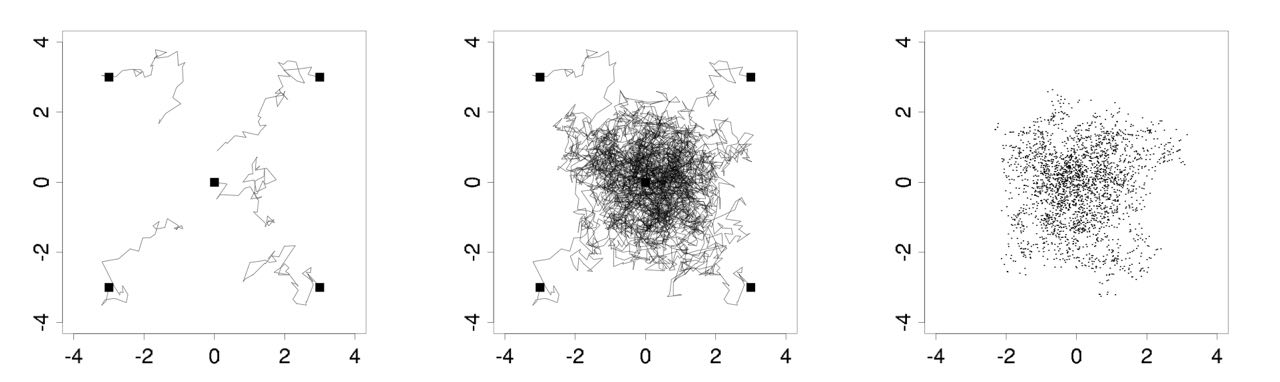
\includegraphics[width=\linewidth]{randomwalk}
\caption{Five different MCMC simulations for a bivariate normal distribution, with starting points marked by black squares. Left: After 50 iterations no convergence is yet to be seen. Middle: After 1000 iterations the chains are closer to convergence. Right: Removing the first halve of simulation draws leaves a set of draws from the target distribution. Taken from \cite{bayes}}
\label{fig:ex}
\end{figure}
\subsubsection{\textsc{Hamiltonian} Monte-Carlo (HMC) and No-U-Turn-Sampling (NUTS)}
The random walk behavior of the \textsc{Metropolis-Hastings} algorithm can make computation of complex models very inefficient \cite{bayes}, therefore more sophisticated methods have been developed. \textsc{Hamiltonian} Monte-Carlo (HMC) \cite{hmc} is an elaborate algorithm that allows to explore the parameter space much more efficient than a simple random walk. It will be described qualitatively in the following, for a detailed discussion see e.g. reference \cite{bayes}. At the heart of the HMC algorithm lies an accept-reject step that is similar to the \textsc{Metropolis-Hastings} algorithm. To arrive at new proposals $\btheta^*$ at step $t$ in the chain however an additional auxiliary variable $\boldsymbol{\phi}$ is introduced that has the same dimension as the parameters $\btheta$ but is independent of $\btheta$ and the data $y$. Introducing the new parameters leads to the joint posterior \cite{stan} 
\begin{equation}
	\begin{aligned}
		p(\btheta,\boldsymbol{\phi}|y)&=p(\btheta|y)\cdot p(\boldsymbol{\phi}|\boldsymbol{\theta},y)=p(\boldsymbol{\phi})\\
		\Leftrightarrow-\log p(\btheta,\boldsymbol{\phi}|y)&=-\log p(\btheta|y)-\log p(\phi)\\
		\overset{\text{Def.}}{\Leftrightarrow} H(\btheta,\boldsymbol{\phi}) &:=V(\boldsymbol{\theta})+T(\boldsymbol{\phi}), 	
	\end{aligned}
\end{equation} 
where in the last step the artificial \textsc{Hamiltonian} $H$ has been introduced as a sum of kinetic energy $T$ and potential $V$. Usually, one chooses $p(\boldsymbol{\phi})$ to be a multivariate normal centered at $0$ with covariance matrix $M$ \cite{bayes}. Applying the well known equations of motion to this \textsc{Hamiltonian} one finds 
\begin{align}
	\frac{\text{d}\theta_i}{\text{d}t}=\frac{\partial H}{\partial \phi_i}=\frac{\partial T}{\partial \phi_i} && \frac{\text{d}\phi_i}{\text{d}t}=-\frac{\partial H}{\partial \theta_i}=-\frac{\partial V}{\partial \theta_i}.
\end{align}
This allows the simultaneous direct numerical integration to evolve \enquote{position} and \enquote{momentum} in $L\cdot\epsilon$ discrete time steps with the so-called \emph{Leap-Frog} algorithm \cite{leapfrog}. Consequently $L$ is called the number of Leap-Frog steps and $\epsilon$ is the scale on which the time is discretized. After performing $L$ Leap-Frog steps a proposal $\left(\btheta^*,\boldsymbol{\phi}^*\right)$ is fed into a \textsc{Metropolis-Hastings} accept-reject step that is then used to update the current parameter value in the \textsc{Markov} chain at position $t$. The auxiliary momentum is discarded because it is drawn anew at the next iteration from its posterior distribution $p(\boldsymbol{\phi})$. When tuned right, the HMC algorithm allows for a rapid exploration of the parameter space \cite{bayes}. An extension of HMC that adaptively determines the number of Leap-Frog steps, the step size $\epsilon$ and covariance matrix $M$ is given by the No-U-Turn-Sampler (NUTS) \cite{nuts}. The number of Leap-Frog steps $L$ is determined individually for each chain iteration $t$; as soon as the distance between the original set $\left(\btheta^{(t-1)},\boldsymbol{\phi}^{t-1}\right)$ and the proposals $\left(\btheta^*,\boldsymbol{\phi}^*\right)$ decreases (i.e. the trajectory makes a U-Turn in parameter space) the Leap-Frog integrator is stopped. The step size $\epsilon$ and covariance matrix $M$ are determined during the warm-up phase and then kept fixed for all iterations that are saved for posterior inference \cite{bayes}.
\subsection{Diagnosing convergence of \textsc{Markov}-chains}

\subsection{Combining inferences}
\label{subsec:combinf}



\subsection{Posterior predictive checks}

\subsection{Choosing a prior}
\subsection{Comparison of \textsc{Bayesian} and Frequentist approach}
\subsubsection{Frequentist Approach}
The traditional approach to this fitting problem is a $\chi^2$ fit. Assume there are $N$ precise predictors $\{x_i\}$ and corresponding measurements $\{y_i\}$ with measurement errors $\{\sigma_i\}$. Additionally, the data $y$ is expected to follow a functional $y=f(x,\boldsymbol{\theta})$ with parameter(s) $\boldsymbol{\theta}$ and predictors $x$. Then the test statistic \begin{equation}
	\chi^2=\sum_{i=1}^{N}\left[\frac{y_i-f(x_i;\boldsymbol{\theta})}{\sigma_i^2}\right]
\end{equation}
can be minimized with respect to the parameters $\boldsymbol{\theta}$ giving according estimates with error bars which are calculated using error propagation from the original data points $\{y_i\}$. The minimization can be solved analytically in the case of linear functions by solving the equation system $$\frac{\text{d}}{\text{d}\boldsymbol{\theta}}\chi^2=0$$
and otherwise numerically. The minimization of $\chi^2$ to get best-fit estimates for the desired parameters can be motivated if one considers the likelihood $\mathcal{L}$ that the data follow the function $f$. It is given by \begin{equation}
	\ln\mathcal{L}=-\frac{1}{2}\sum_{i=1}^N\left[\frac{y_i-f(x_i;\boldsymbol{\theta})}{\sigma_i}\right]^2-\sum_{i=1}^N\ln\sigma_i\sqrt{2\pi},
\end{equation}
if one assumes \textsc{Gaussian} errors at each data point. To maximize the (log-) likelihood with respect to all parameters is then equivalent to minimizing $\chi^2$. As a byproduct, the $\chi^2$ fit also gives a goodness of fit estimate which is given by $\chi^2/\text{NDF}\approx 1$, where $\text{NDF}$ are the number of degrees of freedom. Significantly smaller or larger values indicate too small error estimates or a bad fit, respectively. \cite{statistics}
\subsubsection{Bayesian approach}
As an alternative
\section{Current data situation}

\section{Motivation and Structure of this Thesis}
bla
